\hypersetup{pdfborder=0 0 0}


%-------------------------------------------------------------------------------------
\section{Comparison of solitary waves and associated signal from in situ data}
\label{sectionCampagne}

\subsection{Field campaign Gibraltar 2020 overview}
The field campaign of in situ measurements Gibraltar2020 was carried out by SHOM (and other labs) in fall 2020 in the Strait of Gibraltar and west Alboran aboard the research and survey ship \textit{L'Atalante}. On site measures were taken by ship-based instruments from 8/10/2020 to 20/10/2020. Among those, sampling of the water column at both end of the Strait were realized at the eastern end of the Strait on the 14th and 15th october, and at its western end on the 16th of october.

Additionally, five moorings were deployed as presented in table \ref{tab_moor}, locations are also indicated in figure \noparref{fig_moor}.b. Mooring M1 is positioned west of the slope of Camarinal Sill. Mooring M3 is placed in the western deep half of CS while M2 is positioned in a shallow area at the center. M4 and M5 are positioned near each other at some distance east of CS. Three of the moorings (M1, M3 and M5) are equipped with CTD sensors and the other two (M2 and M4) with ADCP sensors. Sampling frequency range from tens of seconds to one minute.


\begin{table}[!h]
        \centering
        \begin{tabular}{|c|c|c|c|}
                \hline
                 & type & position(deg minute) & time \\ 
                 \hline
                M1 & hydro & N35 55.264 W005 46.739 & 8/10/2020 15h - 9/11/2020 12h\\
                M2 & couranto & N35 55.761 W005 45.288 & 8/10/2020 5h - 17/10/2020 15h\\
                M3 & hydro & N35 54.719 W005 44.459 & 8/10/2020 13h - 22/10/2020 21h\\
                M4 & couranto & N35 55.870 W005 41.020 & 8/10/2020 7h - 17/10/2020 14h\\
                M5 & hydro & N35 56.229 W005 41.026 & 8/10/2020 9h - 1/11/2020 14h\\
                \hline
        \end{tabular}
        \captionof{table}{Type of measures, coordinates and date of deployment for moorings of Gibraltar 2020 field campaign.}
        \label{tab_moor}
        %\end{minipage}
\end{table}

In section \ref{section_obs_moor}, mooring data from M2, M4 and M5 are analyzed for a first observation period covering 8/10 to 18/10, when as indicated in table \ref{tab_moor}, both types of moorings data are available.


\subsection{Insights from VHR simulation as help in preparation of Gibraltar 2020}

The numerical simulations presented in section \ref{sectionSim3D} use a high-resolution, non-hydrostatic model. The field of standard deviation of parameter Q and trace of hydraulic jump in figure (\noparref{fig_moor}.B) is issued from those simulations. In combination with external restrictions such as the dense maritime traffic, strong currents and steep slopes of the area, such diagnosis and others were studied to chose mooring deployment as well as transect plans (not shown).

For exemple, M1 was positioned down the western slope of the sill downflow of a potential primary instability generation area (see section \ref{PartDiag3D} and \ref{section3DResFlow} for a discussion of this diagnosis in high-resolution numerical simulation).

Figure \ref{fig_SARIES} features a comparison between a SAR image of the Strait of Gibraltar with the surface signature of a propagating ISW between CS and the longitude of Tarifa, and the corresponding field of norm of the gradient of surface currents in SimIT showing a travelling wave at approximately the same coordinates. While the shape of the train istelf is different, it can be considered that the simulation gives an accurate idea of teh order of propagation speed of ISWs in the Strait of Gibraltar. This was used to predict position of ISW in relation to the tidal cycle as precdicted by harmonic prediction  (not shown). It was accurate at least in the Strait of Gibraltar itself. In the Alboran Sea, where the influence of the gyre is great on the form of the wave packet, prediction was not as accurate. 

Beyond the propagation speed, the high-resolution of the model means that the shape itself of the train of ISWs is accurate. This is used in the following section \ref{section_obs_moor} to help in the interpretation of mooring data from M4 and M5.

\begin{figure}[!h]
% \centering
 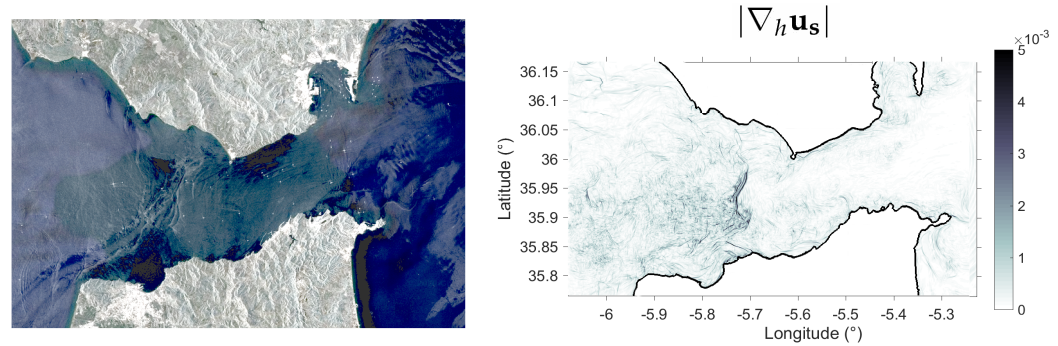
\includegraphics[width=\textwidth]{./GBR3D/Comp_SAR_IES.png}
 \caption {(a) Sentinel-1 Synthetic Aperture Radar (SAR) image (12/09/2017 - 6h18pm UTC). (b) Norm of the gradient of surface horizontal velocity (s-1) in the simulation SimIT (12/09/2017 - 6h30pm or t = 35h30 in simulation time) presented in section \ref{sectionSim3D}.}
 \label{fig_SARIES}
\end{figure}




\subsection{General points on mesoscale circulation during observation period}

\begin{figure}[!h]
% \centering
 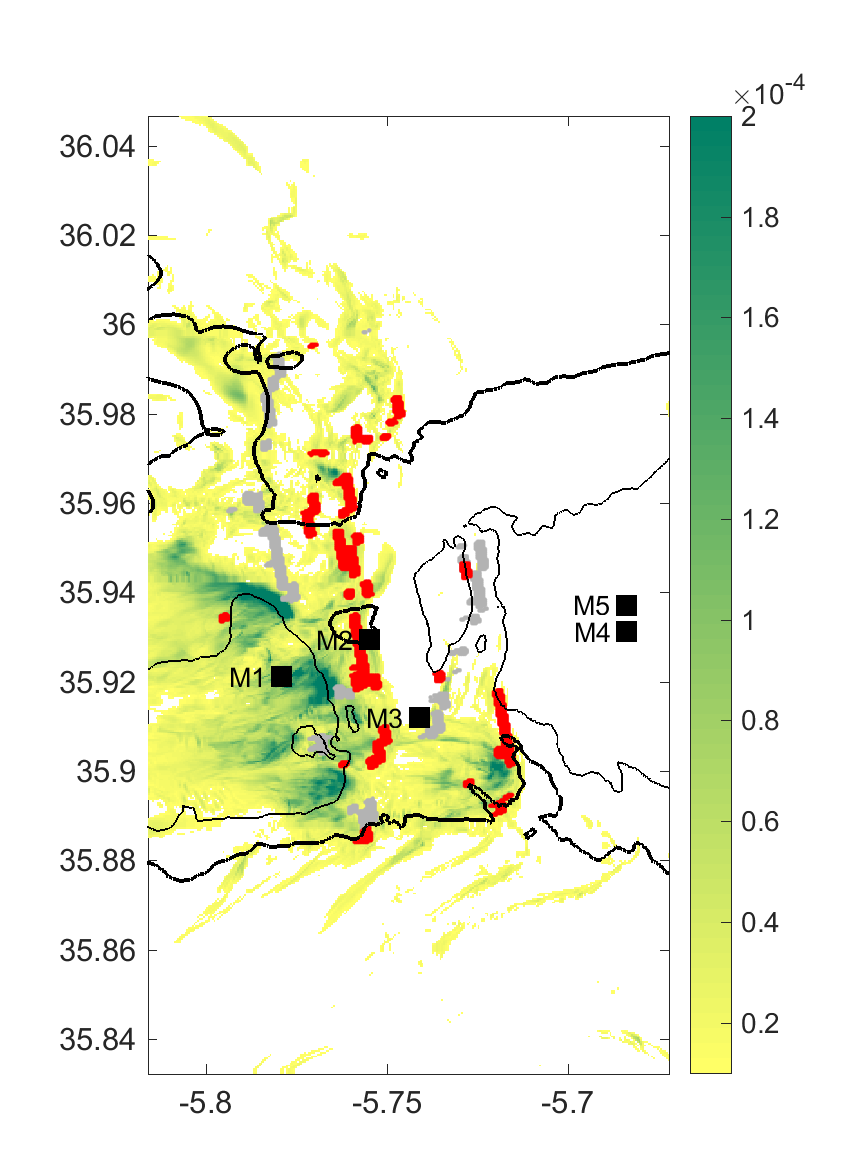
\includegraphics[width=\textwidth]{./GBR3D/Fig_Moor.png}
 \caption {Locations of moorings deployed during Gibraltar 2020 (black squares), over map of standard deviation of parameter Q (colorbar) and location of hydraulic jump of w-type and s-type from high-resolution numerical modelling of the Strait of Gubraltar, as presented in section \ref{sectionSim3D}.}
 \label{fig_moor}
\end{figure}


The in situ time period covers one (for ship-based instruments and ADCP moorings) or two (for CTD moorings) neap-spring tide cycle. Figure \noparref{fig_moor_US3}.b shows the depth-averaged zonal component of current measured at Camarinal Sill from M2 data. The measures begin during the neap tide part of the forthnightly cycle. The west Alboran Gyre was also present in the West Alboran Sea during the field campaign (not shown). 

Figure \noparref{fig_moor}.c and d presents the $\theta$-S diagram from ship-based water column sampling. For both figures, each color refers to a different sampling station indicated in figure \noparref{fig_moor}.a.

On the west end of the Strait, no mediterranean water was sampled at the southernmost station and very mixed signal at the northenmost station, delimiting the path of the Mediterranean outflow between 35.7$^{\text{o}}$ and 36$^{\text{o}}$ N. Among the signals of Mediterranean outflow waters, the two most nothern stations that reach depth $<$400m have a signal more mixed with NACW.

On the east end of the Strait, WMDW is found at depth for all stations except the nothernmost. For the next two stations south of the latter, as well as the two southernmost stations, WMDW is mixed with intermediate waters. 

The five northernmost stations' surface waters are fresher waters upwelled from the Iberian coast, the intermediate Mediterranean waters sampled at these stations are also warmer and saltier compared to the signal of the remaining four, which is interpreted as LIW.



\subsection{Observations of solitary waves at M4 and M5 and currents at Camarinal Sill from M2}
\label{section_obs_moor}

\begin{figure}[!h]
% \centering
 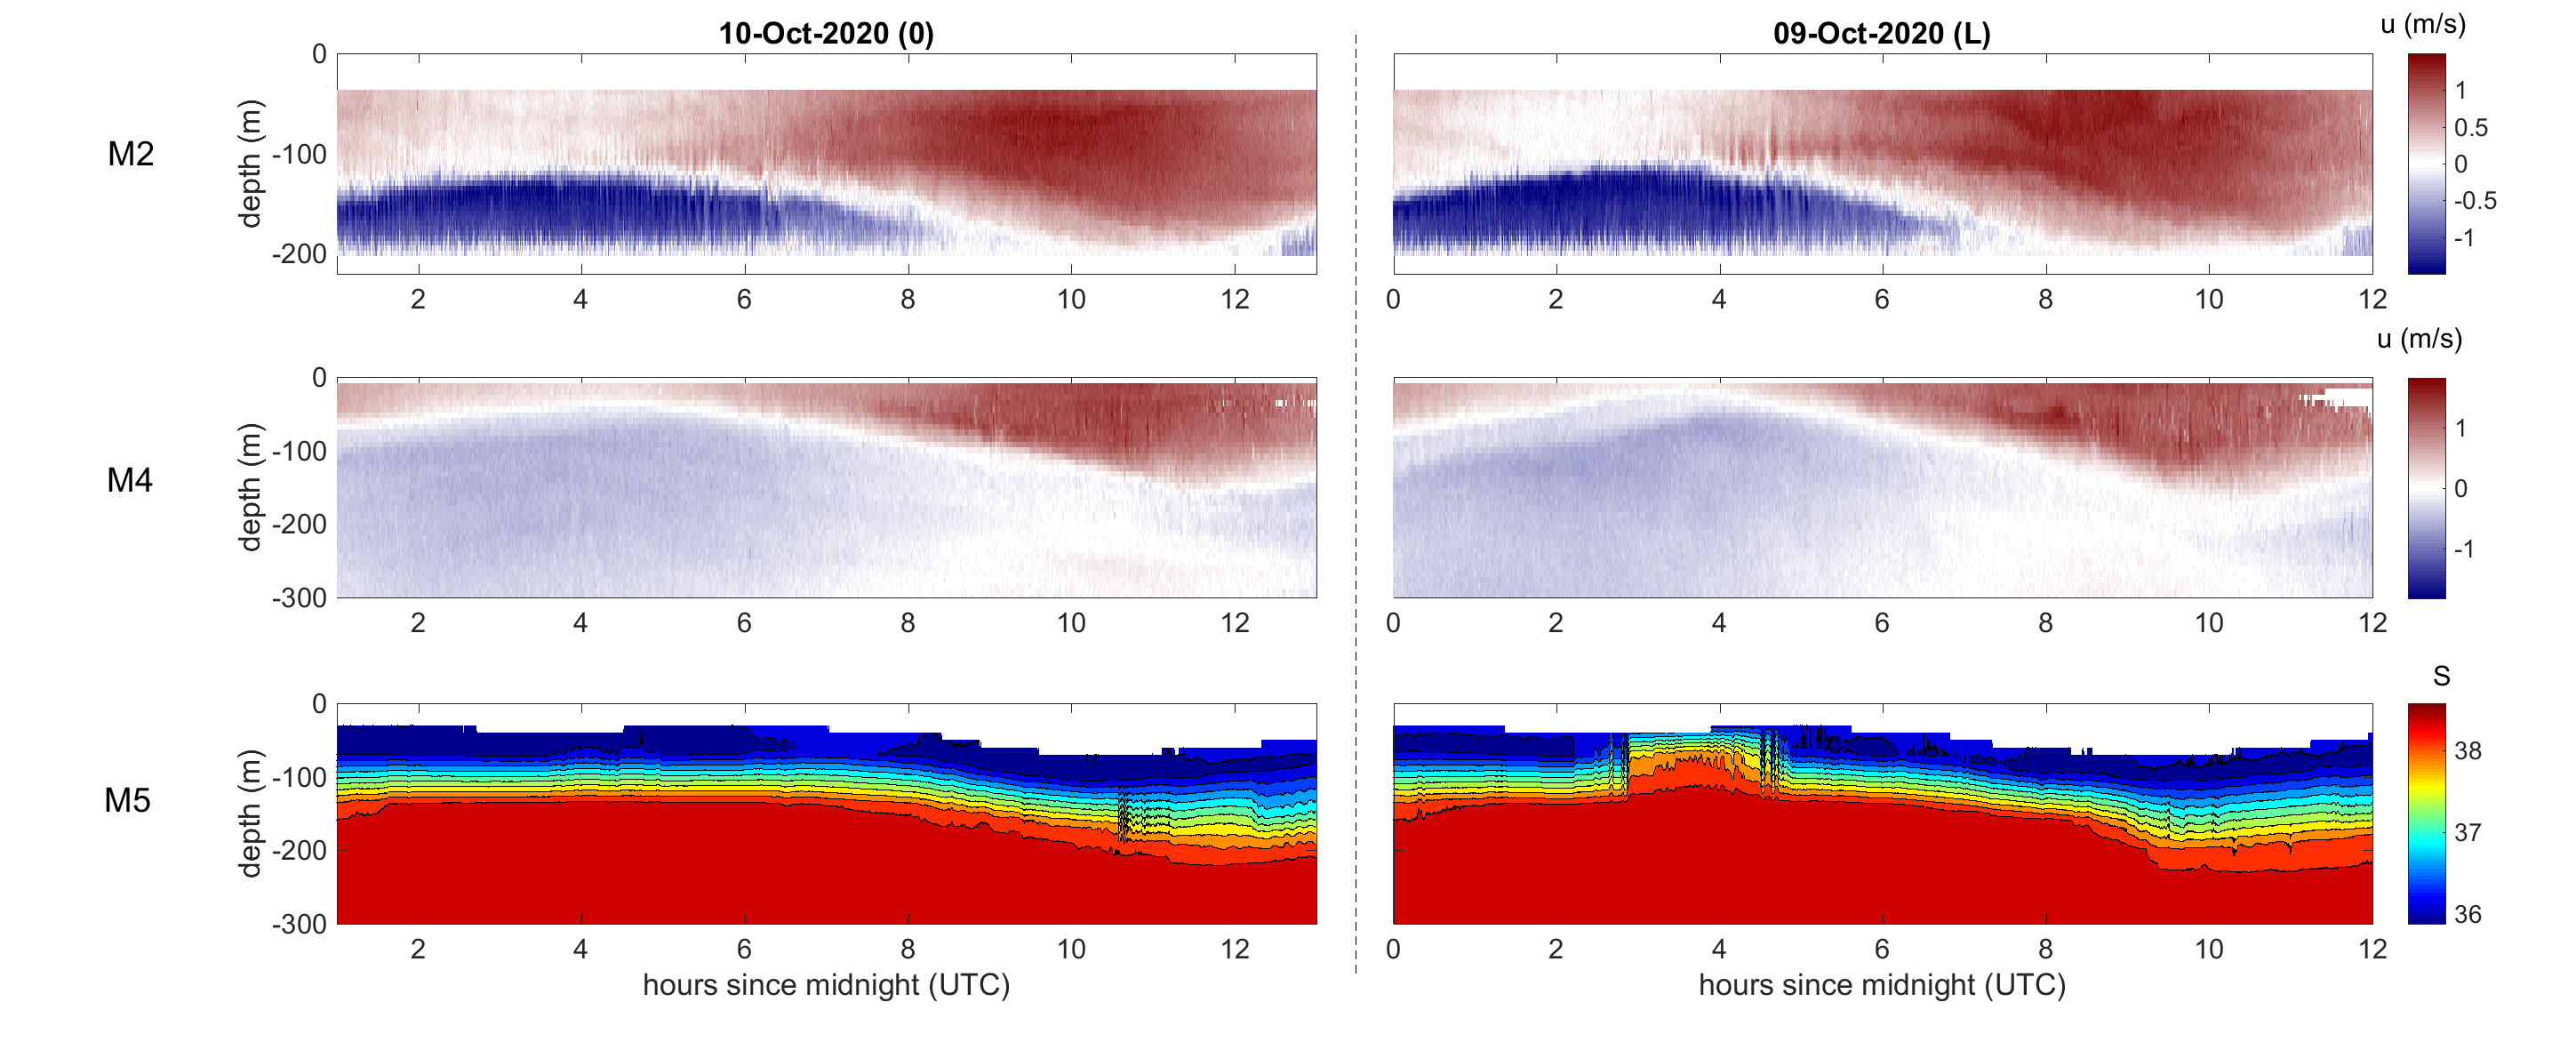
\includegraphics[width=\textwidth]{./GBR3D/US_moorings1.png}
 \caption {Timeseries of moorings data over the water column from M2 (upper row), M4 (center row) and M5 (lower row). The zonal component of currents is represented for M2 and M4 data, and the measured salinity for M5 data.}
 \label{fig_moor_US1}
\end{figure}

\begin{figure}[!h]
% \centering
 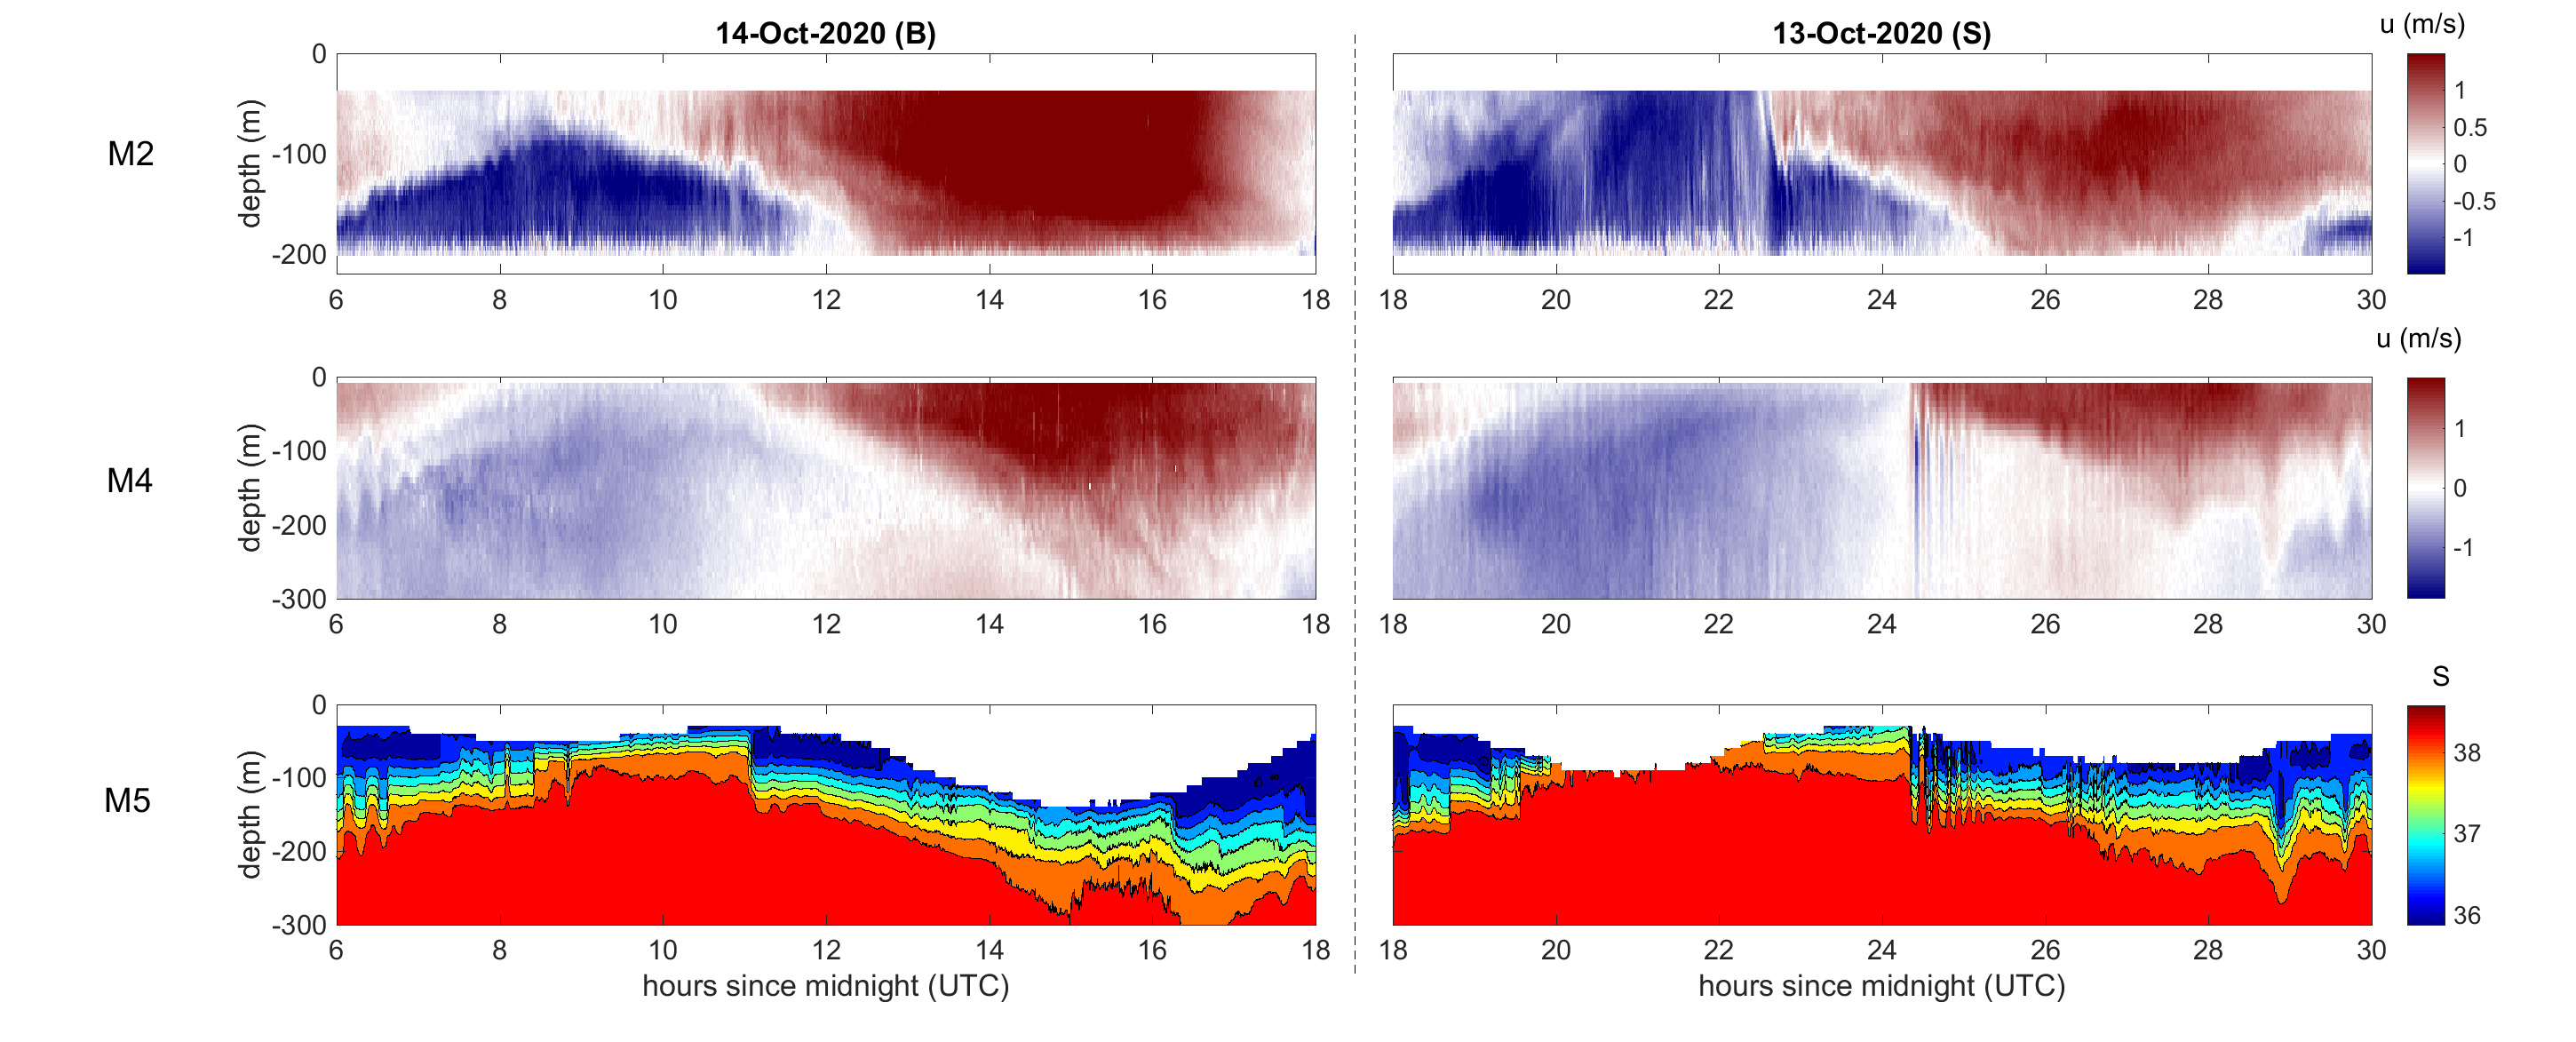
\includegraphics[width=\textwidth]{./GBR3D/US_moorings2.png}
 \caption {Same as figure \ref{fig_moor_US1} for a different time-period.}
 \label{fig_moor_US2}
\end{figure}

\begin{figure}[!h]
% \centering
 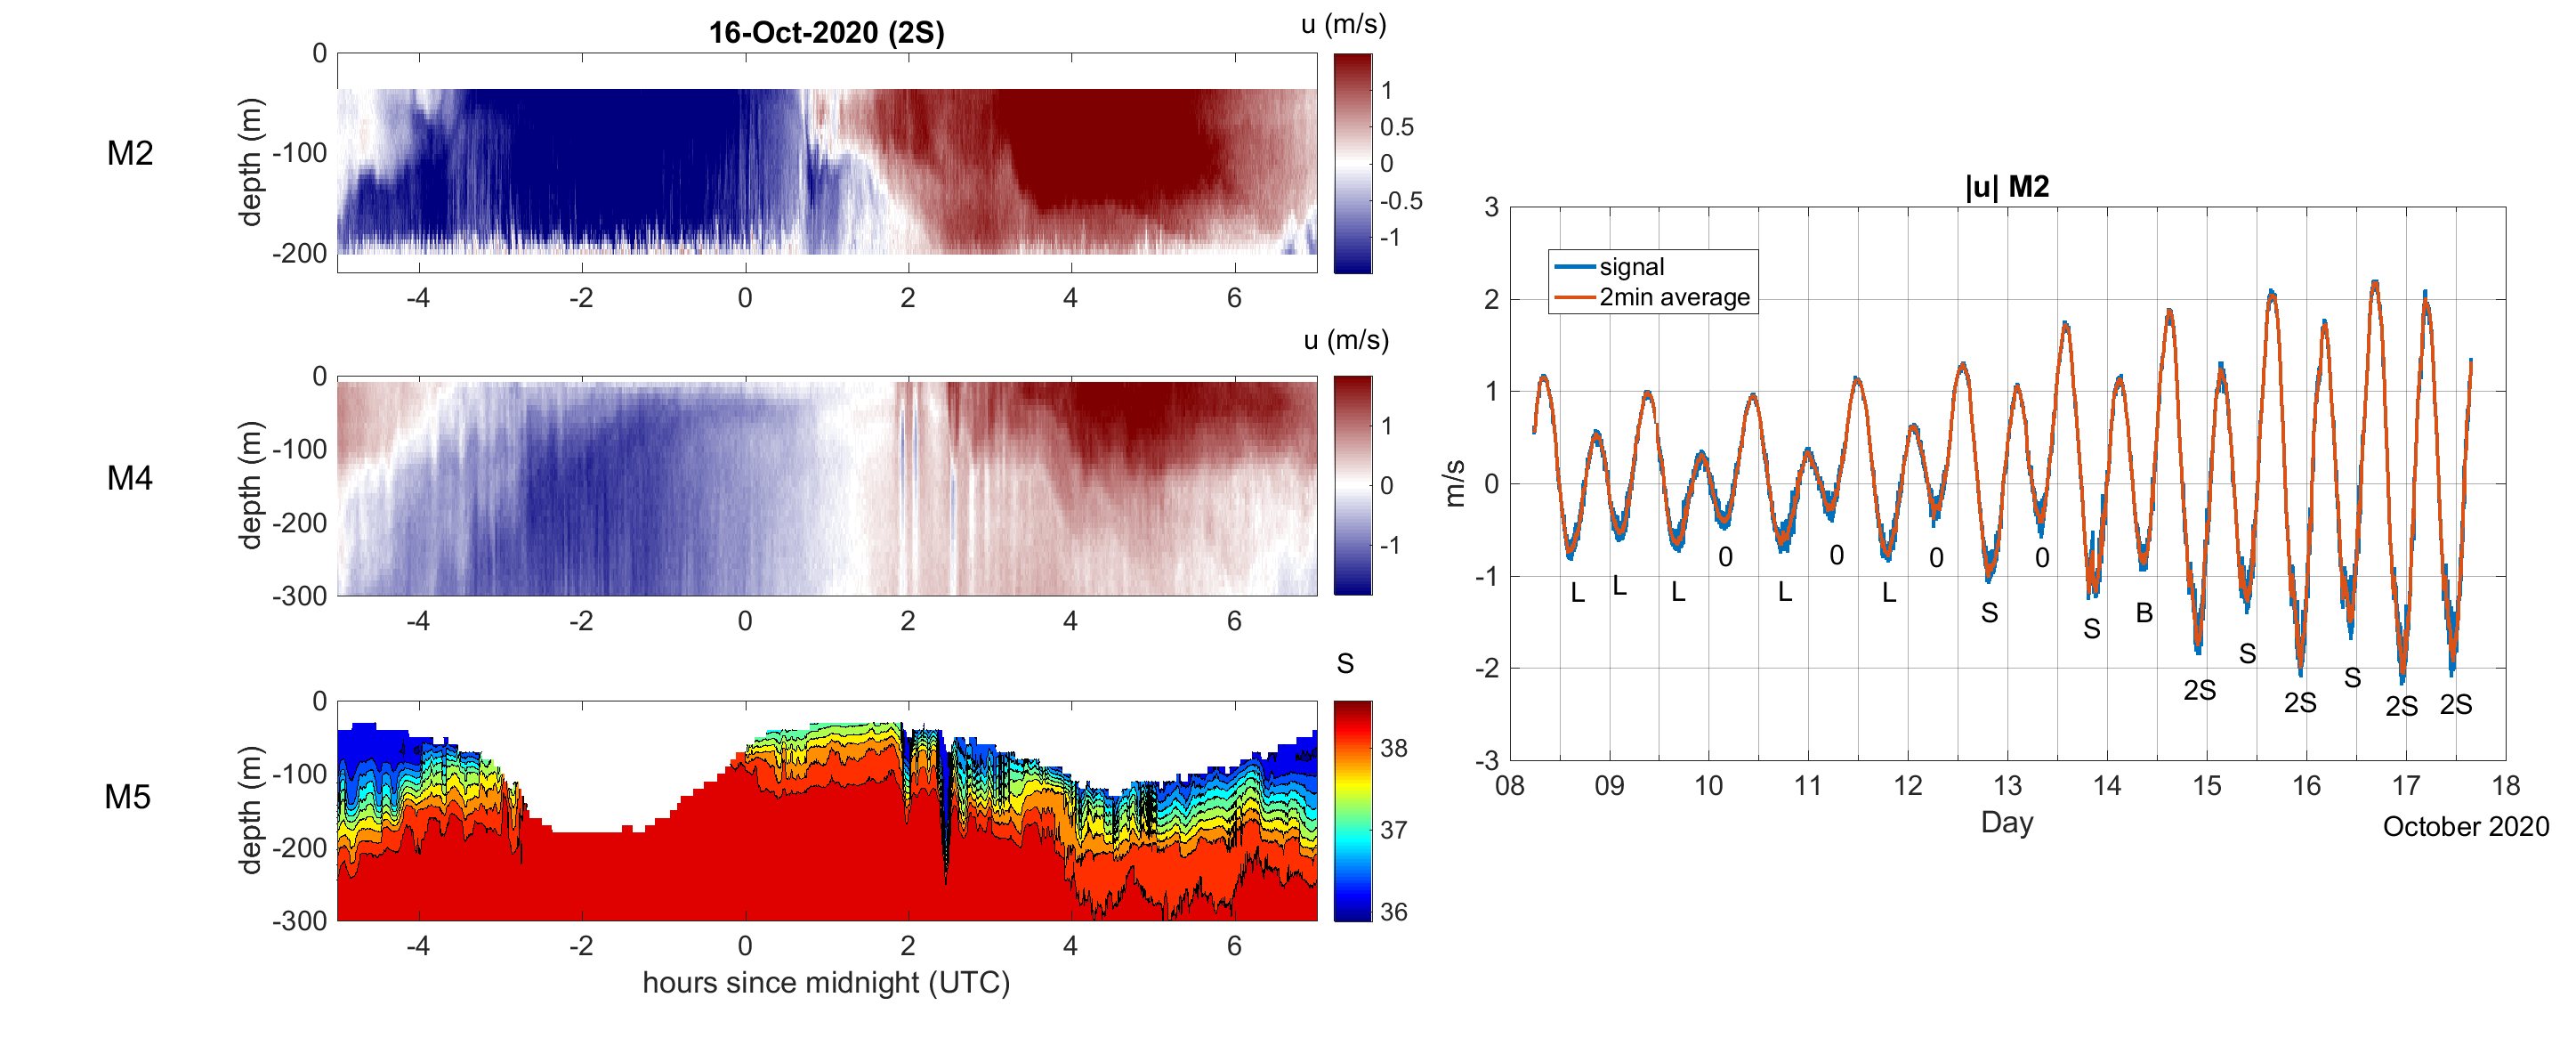
\includegraphics[width=\textwidth]{./GBR3D/US_moorings3.png}
 \caption {(a to c) Same as figure \ref{fig_moor_US1} for a different time-period. (d) Time-serie of depth-Averaged signal of zonal component of currents from M2 data. Each outflow is indicated the type of signal that is observed at M4 and M5.(rajouter SLA tarifa?ou fait trop?)}
 \label{fig_moor_US3}
\end{figure}

Figures \ref{fig_moor_US1} to (\noparref{fig_moor_US3}.A) present depth-time records of the zonal velocity (for M2 and M4 mooring) and salinity (for M5 mooring) for five different M2 tidal periods. Note that while all the water column is presented in those figures for the M2 data, only the upper 300m (of 500m total depth) are represented here for M4 and M5 data for better vizualisation.

Similarly, figure \ref{Fig_moor_USs} presents the zonal velocity and salinity of the upper 300m of simuklated data at a grid point of coordinate (), near M4 and M5, from the simulations SimNT (figure A and B), SimIT (C) and SimST (D) of section \ref{sectionSim3D}. Although those simulations cover a different time-period, the data presents similar patterns of internal waves travelling in the water column to the observed data.


\subsubsection{Currents at M2 and M4}

In the currents data from mooring M2, periods of inflow and outflow can be distinguished respectively as having majoritarly eastward or westward flow over the water column. During inflow, there are always at least two hours during which the whole flow measured by the captors is eastward (for exemple between 10 and 12 hours in figure (\noparref{fig_moor_US1}.A.1)). During outflow, the flow can be westward at all captors, as is the case in figure (\noparref{fig_moor_US2}.B1) and (\noparref{fig_moor_US3}.A1), but this is not necessarily the case. 

In figures (\noparref{fig_moor_US1}.A1) and (B1), for exemple, the baroclinic exchange structure of currents is still distinctive during outflows, with a weak eastward flow in the upper 120m of the water column over a strong current of westward flowing water. Figure (\noparref{fig_moor_US2}.A1) presents another case for which the flow in the upper water column becomes momentarily weakly westward between t=7H and t=9H, with a still clear shear interface at 100m depth.

In the numerical simulations as performed in section \ref{sectionSim3D}, an entirely westward flowing water column at M2 corresponds to an area of supercritical flow for Atlantc waters when an hydraulic jump is present. This location corresponds to the upflow area of the two types of hydraulic jumps identified in section \ref{sectionSim3D}, s-jump and w-jump, and depicted as grey and black points respectively in figure \ref{fig_moor}.

%Those three cases of sheared currents at M2 during outflows happen in the neap-tide part of the forthnight cycle.

At mooring M4, the flow of the water column can become unidirectional for both outflow and inflow periods during the spring tide part of the forthnightly cycle. In this occasions, a shear area still subsists that matches with the salinity interface between mediterranean and atlantic waters in the data of mooring M5 (see for exemple at t=14H in figure (\noparref{fig_moor_US2}.A2) and (A3) between 150-200m depth).

\subsubsection{Observations of propagating high frequency waves}


\begin{figure}[!h]
% \centering
 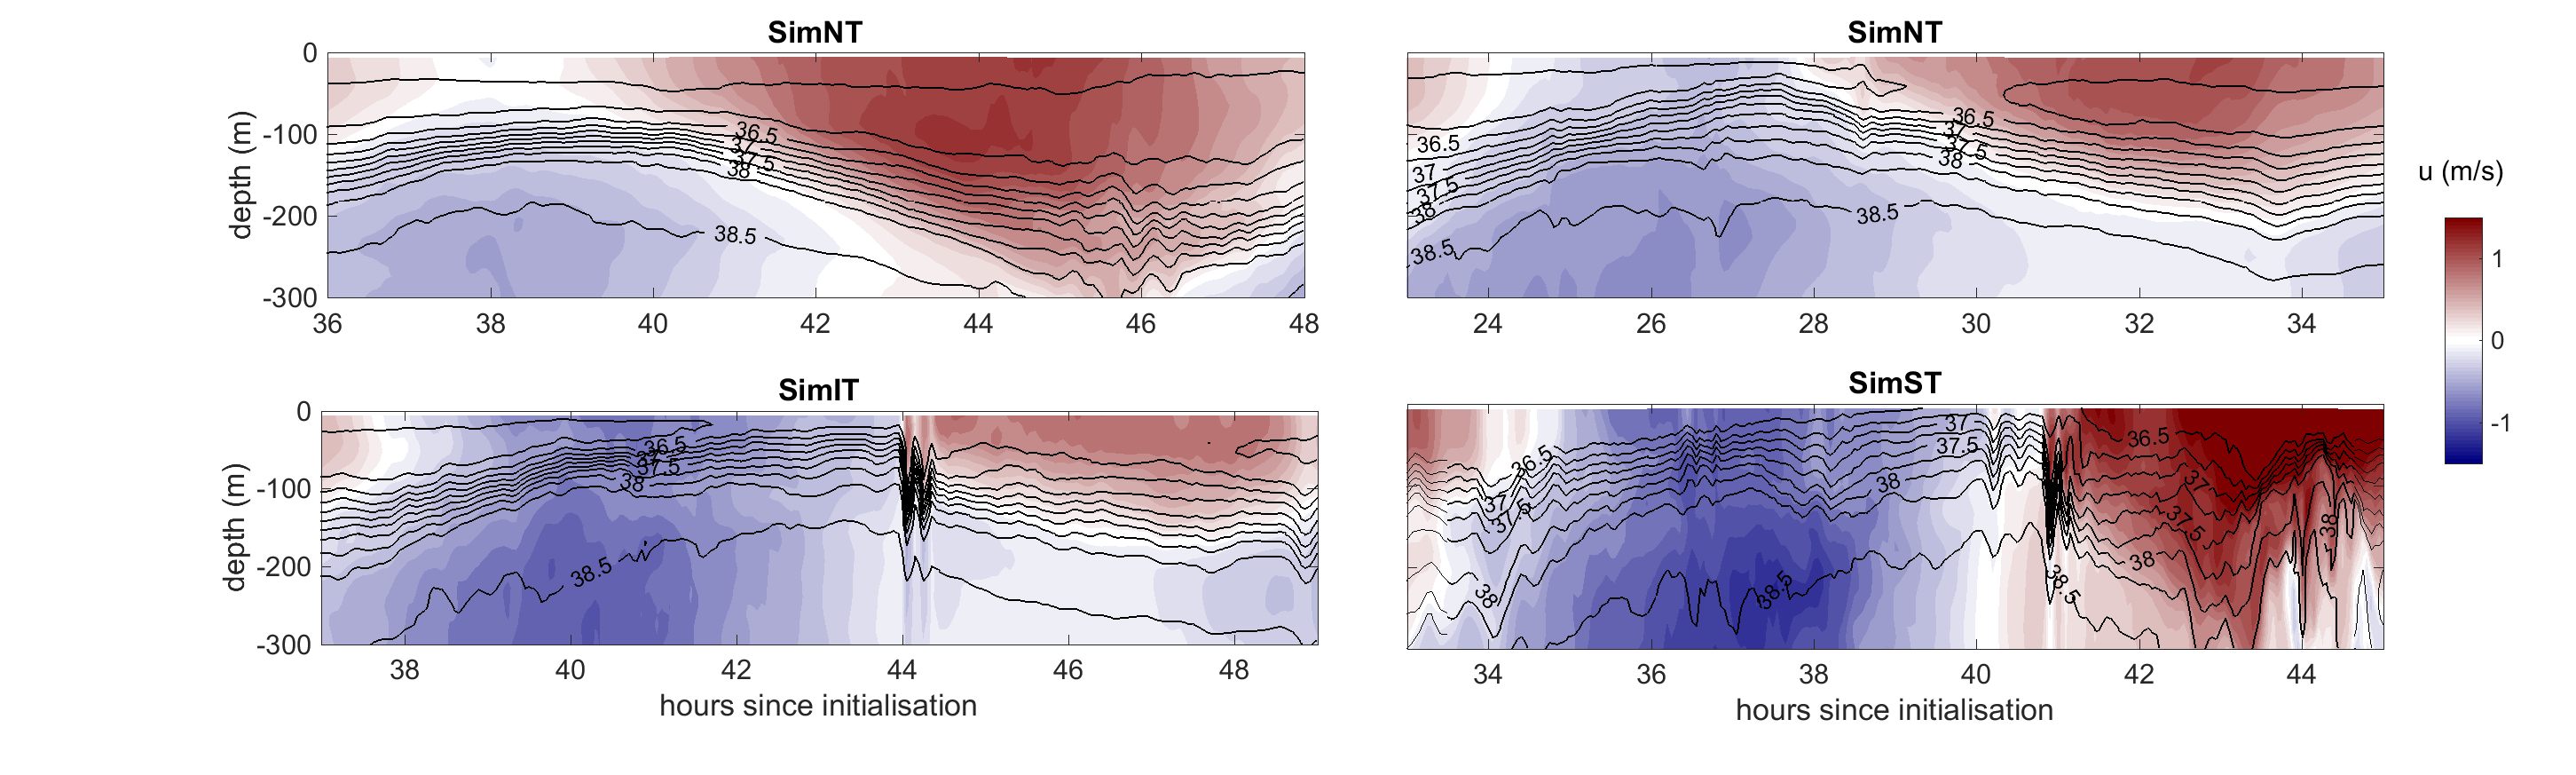
\includegraphics[width=\textwidth]{./GBR3D/US_M4SimMIV.png}
 \caption {Timesieries of salinity (black lines) and zonal velocity (colorbar) in the upper ... m in simulations ... Abscises is simulation time. Mettre des fleches?}
 \label{Fig_moor_USs}
\end{figure}

It is on the salinity interface of M5 data that the signal of propagating internal gravity waves can be spotted, sometimes matching with anomalies in the current field of M4.

In figures (\noparref{fig_moor_US1}.B3) at t=3H, (\noparref{fig_moor_US2}.A3) at t=8H30, and (\noparref{fig_moor_US2}.B3) at t=19h30, show as a recurring feature an abrupt lifting of the interface, that does not appear in the simulations data of figure \ref{Fig_moor_USs}.

Another recurring signal in M5 data are the large amplitude troughs that can be seen during the inflow period of the tidal cycle. In this set it appears clearly in observation data at t=29H in figure (\noparref{fig_moor_US2}.B3). In simulation data (for exemple t=49H in figure (\noparref{Fig_moor_USs}.C)), this signal corresponds to a westward travelling train of ISWs that is generated by reflection of the well-known eastward travelling internal wave train that is generated at Camarinal Sill.

The focus is now made on the signal showing up at M4/M5, usually 3 hours or sooner after the maximal outflow at M2. Five distinctive type of signals are identified and categorized with letters o, L, B, S, and 2S : 

\begin{itemize}
\item \underline{Linear internal tide (o)} : seen in figure (\noparref{fig_moor_US1}.A2) and (A3), for which the depth of the interface of salinity at M5 and maximum shear at M4 evolve linearly, except for some low amplitude tarvelling waves at the interface in M5 at t=10h30. At M2 (figure \noparref{fig_moor_US1}.1.a), there is a distinctive shear in the water column during the preceding outflow, with slightly positive velocity in the upper layer. This signal is also seen in SimNT as shown in figure (\noparref{Fig_moor_USs}.A).
%
\item \underline{Small amplitude internal wave (L)} : seen in figure (\noparref{fig_moor_US1}.B2) and (B3). In the salinty data, there is a signal that looks like two internal waves of relatively small amplitude (10m) at M5 at t=4h30. At M4, the depth of maximum shear of zonal velocity still eveloves in a linear manner as in the (o) case. At M2 in figure (\noparref{fig_moor_US1}.B1), the interface of westward flow evolves at the same depth as in the (o) case but in the above layer velocity becomes almost nil from t=1H to t=3H30. This signal is also seen in SimNT in figure (\noparref{Fig_moor_USs}.B) at t=28.5h of simulation, and is associated here in the velocity field with a mode-1 anomaly.
%
\item \underline{Internal travelling bore (B)} : seen in figure (\noparref{fig_moor_US2}.A2) and (A3). At M5, the salinity interface drops by 50m at t=11H as what looks like a westward propagating internal bore. At M4, however, the maximum shear depth still evolves linearly, but preceding the time of arrival of the internal bore signal, the flow in the water column is negative at all depths. In M2 data at Camarinal Sill, the upper layer velocity is nil or lightly negative during outflow. This type of signal is not seen in the simulations performed.
%
\item \underline{Train of internal solitary waves (S)} : seen in figure (\noparref{fig_moor_US2}.B2) and (B3). A succession of 7 troughs passes at M5 starting t=24h15, teh first one has an amplitude of 80m. In M4, thi serie corresponds to mode-1 anomalies of the velocity field. At M2, the flow throughout the water column is westward, with an abrupt return to a sheared two layer state at t=22h30, corresponding to the loss of hydraulic ontrol and the release of the west hydraulic jump over the Camarinal Sill. In simulations data, this type of signal is seen for exemple in simulation simIT and presented in figure (\noparref{Fig_moor_USs}.C) with two troughs at t=44 H. In simulations, this type of signal at M4/M5 follows the release of a s-jump type of hydraulic jump (ie, at maximum outflow the west hydraulic jump is placed over the shallowest part of CS).
%
\item \underline{Two close trains of internal solitary waves (2S)} : seen in figure (\noparref{fig_moor_US3}.A1) and (A2). Five troughs are seen propagating at M5 starting at t=2H. The first one has an amplitude of 80m and is followed by two short wavelength, small amplitude other troughs, then at t=2h30, an over 100m amplitude new one propagates at M5. It is in turn followed by a smaller-amplitude trough. The mode-1 anomaly of the velocity field is seen clearly at M4 for the first two waves, then the fourth big amplitude one. At M2, as in the previous (S) case, the flow through the water column transitions from wholly westward to sheared two-layer at t=1H. In numerical simulation SimST in figure (\noparref{Fig_moor_USs}.D), four waves are seen that follow this pattern, with a first two waves of decreazing amplitude, then one wave of greater amplitude than the first ones, and another smaller amplitdue wave. In this case, this pattern corresponds to two different trains of ISWs. The first (second) one corresponds to the released previous east (west) hydraulic jump of CS. In the numerical simulations, this signal follows teh release of a w-jump (ie, at maximum outflow the west hydraulic jump is placed over the western slope of CS).
\end{itemize}

S and 2S signals are linked to westward flow of the whole water column at CS, which should indicate that, as in simulation, a hydraulic jump was present west of M2.

In the 2S case seen in simulations, as presented in figure (\noparref{Fig_moor_USs}.D), the amplitude of the first wave linked to the east jump of CS can be very small. It depends on the northern extent/extension (ie, how high a latitude it reaches) of the east hydraulic jump at maximum outflow and the initial angle taken by the released non-linear wave as it first propagates in a slightly south oriented direction.

As the two sets of ISWs propagate further in the Strait, the second train overtakes the first as propagation speed of ISW is linked to amplitude, and they merge into a single train of ISWs. Similarly, the (S) case in simulation appears because the wave released by the west jump of CS overtook the east one sooner due to their initial closeness.

So although they are presented as separate with S following an s-jump and 2S a w-jump in simulations, the possibility must not be excluded that slowly propagating waves from an s-jump could also appear as 2S signal at M4/M5.


\subsection{Remarks on transition between outflow types and ISWs generation in the Strait of Gibraltar}

The classification of the previous section is applied to signals at M4/M5 following each outflow of the first observation period and is marked as annotations in figure (\noparref{fig_moor_US3}.B).

A pattern emerges linking outflow type and strength of the averaged currents at CS. The start of the period corresponds to the neap-tide part of the fortnightly cycle, and either (L) or (o) type of outflows are detected, with no hydraulic jump at CS. The first solitary wave is observed at M4/M5 the 12/10/2020. Due to diurnal inequality of the M2 tide, the next tidal period's outflow is weaker ($<$1m/s) and is an (o) case.

Except for one (B) case the 14/10/2020, for the remaining of the period trains of ISWs (either S or 2S) are propagating through M4/M5. The stronger outflows give (2S) signals since as is expected through numerical simulations of section \ref{sectionSim3D}. Under especially strong outflow the internal hydraulic jump generated over CS is swept downstream as a w-jump, resulting in an initial increased distance between the east and west jump that may not overcome as quickly after release as in the s-jump case. Though as explained previously, for some outflows distinction between S and 2S is subjective.

There is a clear treshold over which begin to have , though stratiication conditions are expected to play an importance in it since it would affect supercriticaity condition for the flow. In numerical simulations, the transition between no solitary waves and solitary waves is expected to be difficult to predict since sensitivity of the system means it relies on good bathymetric feature of the Camarinal Sill to have an accurate strength of the currents, accurate stratification and accurate tidal forcing.

Only one (B) case is observed, it was not featured in numerical simulations so it is less evident whether it can be attributed to an hyraulic jump over CS. While the depth distribution of current at M2 site in the preceding outflow shows a shallower interface and more westward currents in the upper layer than for the (o) and (L) cases, it may be more akin to to a near supercritical flow regime engendering some form of propagating steepening interfacial disturbance.

It was seen in section \ref{section_sim3D_ISW} that even if no hydraulic jump occurs at Camarinal Sill, in numerical simulations at least, the flow of the barotropic tide in the Strait of Gibraltar can lead to a steepening of a long interfacial wave that then develop into a train of ISWs less extensive than in the hydraulic jump case, that propagates in the Alboran Sea. It then is possible that the mechanism of release of the hydraulic jump may not be the only one responsible for generation of observed ISW in the Strait of Gibraltar and the west Alboran Sea. (see \citet{chen_2017} for a summary of various ISW generation mechanisms... (intro + figure 15...point voc))

(Ajouter SAR 6h20 9/10?.... See a propagating wave in Alboran, previously only (L) outflows...)





